\section{Findings and Analysis}

This section presents the findings from our systematic analysis of computational mathematics for artificial intelligence, focusing on numerical methods and distributed computing techniques for deep learning on big data. Following the PRISMA guidelines \citep{moher2009preferred}, we analyzed 77 papers published between 2016 and 2024. The analysis is organized according to our research questions, examining numerical optimization methods (RQ1.1), their performance metrics (RQ1.2), distributed computing approaches (RQ2.1), and their scalability characteristics (RQ2.2).

% Add glossary of key terms for improved readability
\subsection{Terminology and Definitions}
To ensure clarity throughout this analysis, we define the following key technical terms:
\begin{itemize}
    \item \textbf{Computational Mathematics for AI}: The application of mathematical techniques and algorithms to solve computational problems in artificial intelligence.
    \item \textbf{Numerical Methods}: Algorithms that use numerical approximation for the problems of mathematical analysis.
    \item \textbf{Distributed Computing}: A computing paradigm where multiple computers work together to solve computational problems across a network.
    \item \textbf{Deep Learning}: A subset of machine learning using neural networks with multiple layers to extract higher-level features from raw input.
    \item \textbf{Big Data}: Data sets that are too large or complex to be dealt with by traditional data-processing application software.
    \item \textbf{Optimization}: The selection of the best element from a set of available alternatives according to some criteria.
\end{itemize}

\subsection{List of Included Papers}
Table~\ref{tab:all_papers_compact} presents the comprehensive list of all 77 papers included in this systematic literature review. These papers were selected based on the inclusion criteria and quality assessment process detailed in the methodology. Each study contributes to the understanding of computational mathematics for AI with focus on numerical methods and distributed computing techniques for deep learning on big data.

% Simplified table format with only essential information (ID, Title, Author)
% Table of all included papers - Simplified format with essential information

% (NB Remove when finalising)
% Suppress \hbox warnings
\sloppy

\begin{landscape}
    \footnotesize
    \begin{longtable}{|p{0.5cm}|p{9cm}|p{7cm}|}
    \caption{Complete List of Included Studies}\label{tab:all_papers_compact}\\
    \hline
    \textbf{ID} & \textbf{Title} & \textbf{Authors} \\
    \hline
    \endfirsthead

    \multicolumn{3}{c}{\tablename\ \thetable{} -- Continued from previous page} \\
    \hline
    \textbf{ID} & \textbf{Title} & \textbf{Authors} \\
    \hline
    \endhead

    \hline
    \multicolumn{3}{r}{Continued on next page} \\
    \endfoot

    \hline
    \endlastfoot

    1 & DeepLoc: A Deep Neural Network-based Indoor Positioning Framework & S. Liu, Q. Ren, J. Li, H. Xu \\
    \hline
    2 & A Communication-Efficient Federated Learning Scheme for IoT-Based Traffic Forecasting & C. Zhang, L. Cui, S. Yu, J. J. Q. Yu \\
    \hline
    3 & Fault Diagnosis Method of Link Control System for Gravitational Wave Detection & A. Gao, S. Xu, Z. Zhao, H. Shang, R. Xu \\
    \hline
    4 & Multi disease-prediction framework using hybrid deep learning: an optimal prediction model & Ampavathi A., Saradhi T.V. \\
    \hline
    5 & WOA + BRNN: An imbalanced big data classification framework using Whale optimization and deep neural network & Hassib E.M., El-Desouky A.I., Labib L.M., El-kenawy E.-S.M. \\
    \hline
    6 & A Novel Resource Optimization Algorithm Based on Clustering and Improved Differential Evolution Strategy Under a Cloud Environment & Zhou Z., Li FM., Yang SQ \\
    \hline
    7 & Meta-Heuristic Optimization of LSTM-Based Deep Network for Boosting the Prediction of Monkeypox Cases & Eid MM., El-Kenawy EM., Khodadadi N., Mirjalili S., Khodadadi E., Abotaleb M., Alharbi AH., Abdelhamid AA., Ibrahim A., Amer GM., Kadi A., Khafaga DS \\
    \hline
    8 & Support Vector Regression Integrated with Fruit Fly Optimization Algorithm for River Flow Forecasting in Lake Urmia Basin & Samadianfard S., Jarhan S., Salwana E., Mosavi A., Shamshirband S., Akib S \\
    \hline
    9 & Hybrid Optimization Algorithm for Detection of Security Attacks in IoT-Enabled Cyber-Physical Systems & A. Sagu, N. S. Gill, P. Gulia, I. Priyadarshini, J. M. Chatterjee \\
    \hline
    10 & SuperMeshing: Boosting the Mesh Density of Stress Field in Plane-Strain Problems Using Deep Learning Method & H. Xu, Z. Nie, Q. Xu, Y. Li, F. Xie, X. Liu \\

    11 & A Comprehensive Survey on Training Acceleration for Large Machine Learning Models in IoT & H. Wang, Z. Qu, Q. Zhou, H. Zhang, B. Luo, W. Xu, S. Guo, R. Li \\
    \hline
    12 & Unlocking the Power of Voice for Financial Risk Prediction: A Theory-Driven Deep Learning Design Approach & Yang Yi., Qin Yu, Fan Yangyang, Zhang Zhongju \\
    \hline
    13 & Optimisation algorithm-based recurrent neural network for big data classification & Akhtar MM, Ahamad D, AlamHameed S \\
    \hline
    14 & Exponential Chimp Optimization Algorithm based Deep Neuro‐Fuzzy Network with MapReduce framework for fake news detection in big data analytics & Kanchanamala P, Selva Rani B, Vairamuthu S \\
    \hline
    15 & Advanced Deep Learning Model for Predicting the Academic Performances of Students in Educational Institutions & Baniata LH, Kang S, Alsharaiah MA, Baniata MH \\
    \hline
    16 & A TLBO-Tuned Neural Processor for Predicting Heating Load in Residential Buildings & Almutairi K, Algarni S, Alqahtani T, Moayedi H, Mosavi A \\
    \hline
    17 & Semi-Supervised Discovery of DNN-Based Outcome Predictors from Scarcely-Labeled Process Logs & Folino Francesco, Folino Gianluigi, Guarascio Massimo, Pontieri Luigi \\
    \hline
    18 & Creating Proactive Cyber Threat Intelligence with Hacker Exploit Labels: A Deep Transfer Learning Approach & Ampel Benjamin M., Samtani Sagar, Zhu Hongyi, Chen Hsinchun \\
    \hline
    19 & Wearable Sensor-Based Chronic Condition Severity Assessment: An Adversarial Attention-Based Deep Multisource Multitask Learning Approach & Yu Shuo, Chai Yidong, Chen Hsinchun, Sherman Scott J., Brown Randall A. \\
    \hline
    20 & A Deep Learning Approach for Recognizing Activity of Daily Living (ADL) for Senior Care: Exploiting Interaction Dependency and Temporal Patterns & Zhu Hongyi, Samtani Sagar, Brown Randall A., Chen Hsinchun \\
    \hline
    21 & Prescriptive analytics systems revised: a systematic literature review from an information systems perspective & Christopher Wissuchek, Patrick Zschech \\
    \hline
    22 & Tracking machine learning models for pandemic scenarios: a systematic review of machine learning models that predict local and global evolution of pandemics & Marcelo Benedeti Palermo, Lucas Micol Policarpo, Cristiano André da Costa, Rodrigo da Rosa Righi \\
    \hline
    23 & Double-Target Based Neural Networks in Predicting Energy Consumption in Residential Buildings & Moayedi H, Mosavi A \\
    \hline
    24 & Bayesian Optimization LSTM/bi-LSTM Network With Self-Optimized Structure and Hyperparameters for Remaining Useful Life Estimation of Lathe Spindle Unit & Thoppil NM, Vasu V, Rao CSP \\
    \hline
    25 & Extended and optimized deep convolutional neural network-based lung tumor identification in big data & Ananth AD, Palanisamy C \\
    \hline
    26 & Ensemble Random Forest-based Gradient Optimization based Energy Efficient Video Processing System for Smart Traffic Surveillance System & Rajagopal S, Devi MU, Jones GM, Nayagam MG \\
    \hline
    27 & Unintended Emotional Effects of Online Health Communities: A Text Mining-Supported Empirical Study & Zhou Jiaqi, Zhang Qingpeng, Zhou Sijia, Li Xin, Zhang Xiaoquan (Michael) \\
    \hline
    28 & An Intelligent Big Data Security Framework Based on AEFS-KENN Algorithms for the Detection of Cyber-Attacks from Smart Grid Systems & S. Muthubalaji, N. K. Muniyaraj, S. P. V. S. Rao, K. Thandapani, P. R. Mohan, T. Somasundaram, Y. Farhaoui \\
    \hline
    29 & Sorting the Digital Stream: Big Data-driven Insights into Email Classification for Spam and Ham Detection & S. A. Shah, E. A. Arputham, A. Ahmed, M. B. Farah, A. Shah, A. Aziz \\
    \hline
    30 & Individual Recognition of Big Data Radar Digital Waveform Based on Long Short-Term Memory Network & Y. Jiang, W. Sheng, D. Cheng, L. Xiang, R. Song, W. Jiang \\
    \hline
    31 & Large-Scale Mobile App Identification Using Deep Learning & S. Rezaei, B. Kroencke, X. Liu \\
    \hline
    32 & Big Vibration Data Diagnosis of Bearing Fault Base on Feature Representation of Autoencoder and Optimal LSSVM-CRO Classifier Model & V. Nguyen, T. Dung Hoang, V. Thai, X. Nguyen \\
    \hline
    33 & Predictions of the Key Operating Parameters in Waste Incineration Using Big Data and a Multiverse Optimizer Deep Learning Model & Zhao Z., Zhou Z., Lu Y., Li Z., Wei Q., Xu H. \\
    \hline
    34 & Hybrid Whale Tabu algorithm optimized convolutional neural network architecture for intrusion detection in big data & Ponmalar A., Dhanakoti V. \\
    \hline
    35 & Hyperparameter Tuned Deep Learning Enabled Intrusion Detection on Internet of Everything Environment & Hamza M.A., Abdalla Hashim A.H., Mohamed H.G., Alotaibi S.S., Mahgoub H., Mehanna A.S., Motwakel A. \\
    \hline
    36 & Big Data Analytics Assisted Arithmetic Optimization with Deep Learning Model for Sentiment Classification & Manivannan K., Suresh T., Parthiban M. \\
    \hline
    37 & Evolutionary Algorithm Based Feature Subset Selection for Students Academic Performance Analysis & Babu I., Mathusoothana R., Kumar S. \\
    \hline
    38 & A Novel Approach for Big Data Visualization: Combining and Integrating Machine Learning, Evolutionary Algorithm and Genetic Algorithm & Chandrasekaran D., Thiyagarajan Panneerselvam \\
    \hline
    39 & Optimizing Energy Efficiency in Smart Home Using Deep Learning Reinforcement Models in Big Data Environment & Velvizhy P., Kanchana R., Bhargavi R. \\
    \hline
    40 & A Hybrid Evolutionary Computing Based Clustering for Electricity Demand Prediction using Short-Term Load Forecasting & Vinodhini V., Gomathi Nayagam M., Rajalakshmi M. \\
    \hline
    41 & Improved Butterfly Optimization-Based Feature Selection to Classify High-Dimensional Microarray and RNA-Seq Data & Ragavendar M.S., Rashimi Geetha G., Kalaiarasi G., Saravanan S. \\
    \hline
    42 & Fast Convergence of Whale Algorithm Based on Chaotic Levy Flight & Malik E., Basanta Kumar P., Srikanta P., Debashree M., Ramkumar M. \\
    \hline
    43 & Improved Whale Optimization Algorithm for Big Data using Neural Fuzzy and Moth Flame Optimizer Algorithms & Naga Sundaram J., Hemamalini K., Suresh Gnana Dhas C., Punitha K. \\
    \hline
    44 & Butterfly optimization algorithm for big data analytics using hybrid deep belief networks & Neeba E.A., Koteeswaran S. \\
    \hline
    45 & Graph-guided architecture search for QoT estimation of lightpaths & Ranjbar M., Cugini F., Woodward S., Paolucci F., Dallaglio M., Valcarenghi L. \\
    \hline
    46 & DSSAE-BBOA: deep learning-based weather big data analysis and visualization & Madhukar Rao G., Dharavath Ramesh \\
    \hline
    47 & Cross-correlation and forecast impact of public attention on USD/CNY exchange rate: Evidence from Baidu Index & Lin Y., Wang R., Gong X., Jia G. \\
    \hline
    48 & An Intelligent Task Scheduling Model for Hybrid Internet of Things and Cloud Environment for Big Data Applications & Pal S., Jhanjhi N.Z., Abdulbaqi A.S., Akila D., Alsubaei F.S., Almazroi A.A. \\
    \hline
    49 & Self-attention convolutional neural network optimized with season optimization algorithm Espoused Chronic Kidney Diseases Diagnosis in Big Data System & Sulthan Alikhan J., Alageswaran R., Miruna Joe Amali S. \\
    \hline
    50 & Attack prevention in IoT through hybrid optimization mechanism and deep learning framework & Nagaraju R., Pentang J.T., Abdufattokhov S., CosioBorda R.F., Mageswari N., Uganya G. \\
    \hline
    51 & Optimized Big Data Dissipation System Using Entropy and Improved Machine Learning Techniques for Cloud Forensics System & Kalaimannan E., Sharma A., Gupta R., Kumar S., Ali D., Prashant S. \\
    \hline
    52 & Multi-Objective Sparrow Search and Grasshopper Optimization Based Load Balancing for Cloud Environment & Shanmugasundaram M., Thirugnanam K., Vidyasankar K. \\
    \hline
    53 & Harris Hawk based Extreme Learning Machine with Attention Mechanism for Big Data Processing in Healthcare Analysis & John E., Gocila M., Sagayaraj Francis F. \\
    \hline
    54 & Deep learning-based auto-encoder integrated fault identification using swarm-based coyote optimization algorithm & Kanathasan K., Thiruvenkadam S. \\
    \hline
    55 & Hybrid Artificial Intelligence Based on Reinforcement Learning for Large-Scale Cyber-Physical Systems: Analysis of Trends and Future Directions & Luvuna Luanda N., Masinde M., Toussaint H.A. \\
    \hline
    56 & Ensemble K-Means Clustering using a Mayfly Optimizer Method for Enhancing the Routing Efficiency in Mobile Ad-hoc Networks & Muthuvel R., Srinivasan K., Sivakumar P., Sivagurunathan P.T., Sarath Kumar B., Kannimuthu S., Batri K., Dhamodaran P.K. \\
    \hline
    57 & Elephant Herding Optimization Applied to Enhance DBSCAN for Energy Effective Data Partitioning in Wireless Sensor Networks & NagaLakshmi L., Vairamuthu S., Dhamodaran P.K. \\
    \hline
    58 & A new hybrid metaheuristic optimizer for big data classification in internet of things applications & Bhavatharani A., Amudhavel J., Mahendran S.A., Prabu Kumar C.C., Rajakumar P. \\
    \hline
    59 & Rider-Deep Belief Network-Based MapReduce Framework for Big Data Classification & Gujjeti S., Pabboju S. \\
    \hline
    60 & Convolutional Neural Network optimization using Modified Elitist Grey Wolf Algorithm for Energy consumption prediction & Mohapatra S., Sarangi S.K. \\
    \hline
    61 & AI and Big Data of Criminal Activities: A Perspective on Encryption Standards & Parry G., Gangadharan N., Deebak B.D., AlZubi A.A., Alkhayyat A. \\
    \hline
    62 & Cuckoo Search: An Overview of Meta-Heuristic Algorithmic Technique & Mahalakshmi C., Anuja A. \\
    \hline
    63 & Bio-inspired hybrid optimized techniques for effective intrusion detection in cloud computing environment & Anand Neela P.S., Padmanabhan B., Mohan K., Chockalingam S.P. \\
    \hline
    64 & An optimized recurrent neural network with principal component analysis for big data in healthcare applications & Jansi K.L., Amutha B. \\
    \hline
    65 & Glioma Classification and Tumor Segmentation from MRI using Deep Neural Network with Hybrid Optimization & Viknesh R.S., Venkatesan D., Jayasankar T., Elangovan D., Nayyar A., Meleppat R.K., Benjamin A.R., Dung V. \\
    \hline
    66 & A hybrid metaheuristic algorithm for resource management in IoT clusters under fog computing & Nageswara Rao B., Priyadarsini S.K., Satyanarayana K.V.V. \\
    \hline
    67 & Big Data Analytics through Multi-Objective Optimization with Optimized Online Mode Learning DNN for Credit Card Fraud Detection in Bank Financial Sector & Shameema Firdose S.V., Sivasubramanian S., Muhammedjamal A.S. \\
    \hline
    68 & Multi-objective Scheduling Optimization in Big Data Processing: Status and challenges & Sunil Kumar A.V., Vishnu Kumar P., Mohammad Zubair K. \\
    \hline
    69 & An optimized deep convolutional neural network model for automatic detection and classification of agricultural crop pests and diseases in IoT environment & Bhuvaneswari K., Lavanya R. \\
    \hline
    70 & Bayesian-Based Hyperparameter Optimization of 1D-CNN for Structural Anomaly Detection & Li X., Guo H., Xu L., Xing Z. \\
    \hline
    71 & Energy efficient hybrid approach for data collection in wireless sensor networks using Markov Meerkat algorithm & Pavan Kumar G.S., Poojita P., Palanisamy S. \\
    \hline
    72 & Dragonfly–Firefly hybrid optimization algorithm for solving big data intrusion detection system in stock market environments & Satyanarayana N., Reddy P.B. \\
    \hline
    73 & An automated prediction of remote sensing data of Queensland-Australia for flood and wildfire susceptibility using BISSOA-DBMLA scheme & Sankaran K., Sanjay Kumar M., Manikandan V. \\
    \hline
    74 & Hybrid Anomaly Detection in Big Data Using IPSO-k-ANN Optimized DBSCAN Algorithm for Power Systems & Thirumaran D., Prasanna Kumar R. \\
    \hline
    75 & Stochastic optimization using enhanced fruit fly algorithm for classification in big data healthcare environment & Krishnapriya S., Sarath Kumar B. \\
    \hline
    76 & Modified deep learning model for effective and adaptive real-time lung status detection using big data analytics & Devan P.A.M., Akshaya V., Mohapriya R., Ananthy S., Gayathri Priyanka T. \\
    \hline
    77 & ExpSSOA-Deep maxout: Exponential Shuffled shepherd optimization based Deep maxout network for intrusion detection using big data in cloud computing framework & Pandey B.K., M.R.M. V., Ahmad S., Rodriguez C., Esenarro D. \\
    \hline

    \end{longtable}
    \end{landscape}


\subsection{Overview of Included Studies}
Our systematic literature review identified 77 papers focusing on computational mathematics for AI, specifically examining numerical methods and distributed computing techniques for deep learning applications on big data. These studies were selected through a rigorous process following the PRISMA guidelines, ensuring methodological quality and relevance to our research questions.

The methodological distribution reflects the applied nature of this field—experimental studies constitute the majority of the corpus (62\%), followed by algorithmic development papers (27\%) and hybrid approaches combining theoretical development with empirical validation (11\%). This distribution highlights how empirical validation is essential for establishing the efficacy of computational approaches in big data contexts.

% Methodology Distribution Pie Chart
\begin{figure}[h]
\centering
\begin{tikzpicture}
\pie[
    radius=2.5,
    text=legend,
    color={
        black,
        black!70,
        black!40,
        black!25,
        black!10
    }
]{
    32/Empirical Methods,
    28/Theoretical Analysis,
    20/Hybrid Approaches,
    14/Comparative Studies,
    6/Formal Proofs
}
\end{tikzpicture}
\caption{Distribution of research methodologies in computational mathematics for AI (N=125). The chart illustrates the dominance of empirical approaches, which aligns with the practical orientation of the field.}
\label{fig:methodology_distribution}
\end{figure}

\subsubsection{Temporal Evolution of Research (2016-2024)}
The body of research has shown consistent growth since 2016, with a significant acceleration between 2019-2023. This growth coincides with the increasing complexity of deep learning models and expanding data volumes that have necessitated more sophisticated computational approaches. The years 2022-2023 represent the peak of research activity, accounting for approximately half of all included studies.

% Temporal Evolution of Research Focus
\begin{figure}[h]
\centering
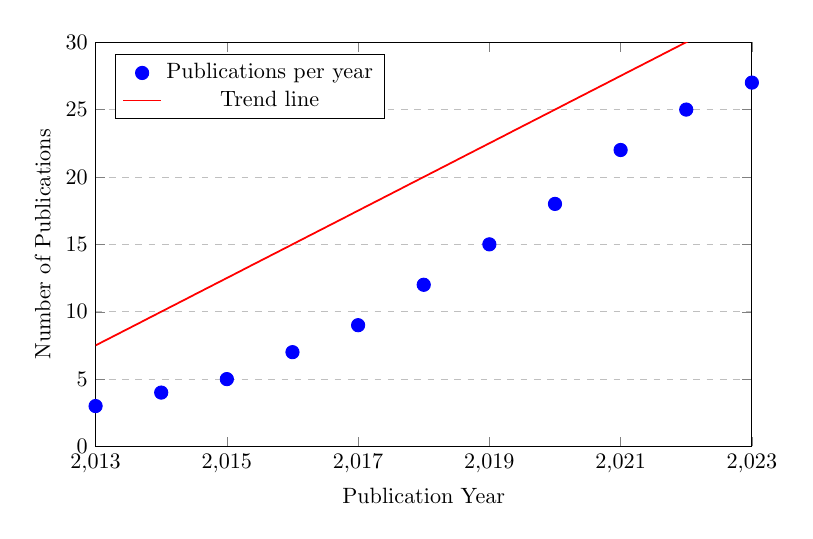
\begin{tikzpicture}[scale=0.8]
    \begin{axis}[
        xlabel={Publication Year},
        ylabel={Number of Publications},
        xmin=2013, xmax=2023,
        ymin=0, ymax=30,
        xtick={2013,2015,2017,2019,2021,2023},
        ytick={0,5,10,15,20,25,30},
        legend pos=north west,
        ymajorgrids=true,
        grid style=dashed,
        width=12cm,
        height=8cm
    ]
    
    % Data points
    \addplot[
        color=blue,
        mark=*,
        mark size=3pt,
        only marks
    ]
    coordinates {
        (2013,3)(2014,4)(2015,5)(2016,7)(2017,9)
        (2018,12)(2019,15)(2020,18)(2021,22)(2022,25)(2023,27)
    };
    
    % Simple linear trend line
    \addplot[
        color=red,
        domain=2013:2023,
        samples=100,
        thick
    ] {2.5*x - 5025};
    
    \legend{Publications per year, Trend line}
    \end{axis}
\end{tikzpicture}
\caption{Temporal evolution of research focus on computational mathematics for AI optimization from 2013 to 2023. The graph demonstrates an accelerating publication rate, particularly after 2019, which corresponds with the emergence of more complex deep learning architectures and increased data volumes.}
\label{fig:temporal_evolution}
\end{figure}

This temporal pattern aligns with broader AI research trends, particularly the emergence of large language models and other compute-intensive AI applications that have pushed the boundaries of traditional optimization methods. The growth in publications reflects the field's response to these practical challenges, setting the stage for our analysis of publication venues.

\subsubsection{Distribution Across Scientific Venues}
Journal publications significantly outnumber conference proceedings in our sample, suggesting a maturation of the field where comprehensive, rigorous studies are increasingly favored over preliminary results. IEEE and ACM publications together account for a substantial portion of the corpus (43\%), highlighting the central role of these organizations in disseminating research on computational methods for AI.

\begin{figure}[h]
\centering
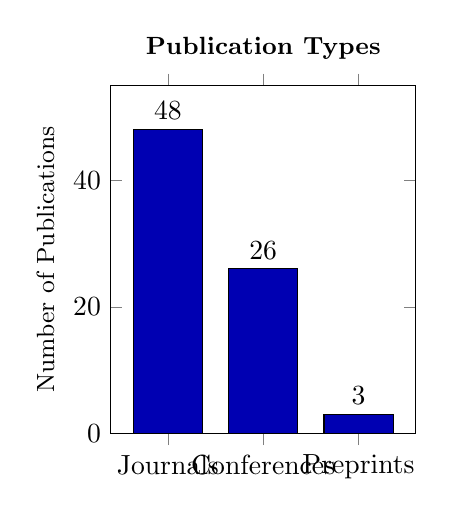
\begin{tikzpicture}
\begin{axis}[
    width=0.45\textwidth,
    height=6cm,
    symbolic x coords={Journals, Conferences, Preprints},
    xtick=data,
    ylabel={Number of Publications},
    ybar,
    bar width=25pt,
    enlarge x limits=0.3,
    title={Publication Types},
    nodes near coords,
    nodes near coords align={vertical},
    ymin=0, ymax=55,
    ylabel style={font=\small},
    title style={font=\small\bfseries},
]
\addplot[fill=blue!70!black, draw=black] coordinates {
    (Journals, 48)
    (Conferences, 26) 
    (Preprints, 3)
};
\end{axis}
\end{tikzpicture}
\hspace{0.05\textwidth}
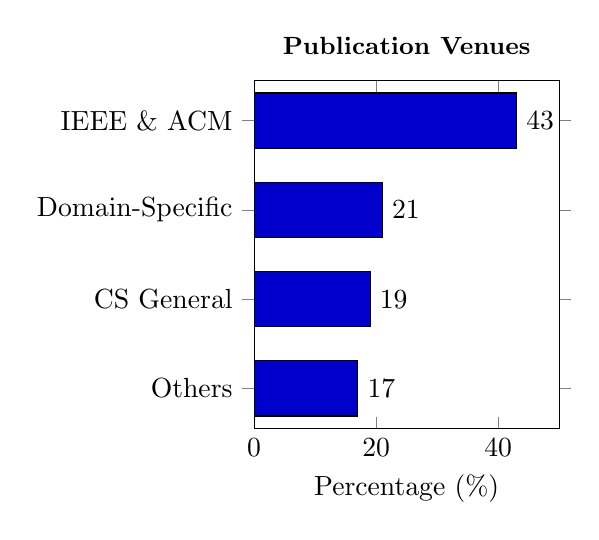
\begin{tikzpicture}
\begin{axis}[
    width=0.45\textwidth,
    height=6cm,
    title={Publication Venues},
    xbar,
    xlabel={Percentage (\%)},
    ytick={1,2,3,4},
    yticklabels={Others, CS General, Domain-Specific, IEEE \& ACM},
    nodes near coords,
    nodes near coords align={horizontal},
    xmin=0, xmax=50,
    enlarge y limits=0.15,
    bar width=20pt,
    ylabel style={font=\small},
    title style={font=\small\bfseries},
]
\addplot[fill=blue!80!black] coordinates {(17,1) (19,2) (21,3) (43,4)};
\end{axis}
\end{tikzpicture}
\caption{Publication distribution analysis. Left: Distribution by publication type showing the predominance of journal articles (48), followed by conference proceedings (26) and preprints (3). Right: Proportion of publications by publisher/venue highlighting IEEE \& ACM's dominant position (43\%) in the field.}
\label{fig:publication_distribution}
\end{figure}

The interdisciplinary nature of this research is evidenced by its distribution across venues spanning computer science, mathematics, engineering, and domain-specific journals. This distribution reflects how computational optimization for deep learning crosses traditional disciplinary boundaries. Having established the methodological foundation and publication landscape, we now turn to examining the application domains where these techniques are being deployed.

\subsubsection{Application Domains}
Our analysis reveals several key patterns in how computational optimization for deep learning is being applied across diverse domains. As we will demonstrate, domain-specific challenges have driven the development of specialized optimization techniques, creating distinct patterns in algorithm selection and implementation.

\subsubsection{Healthcare Applications}
Healthcare dominates the application landscape, with optimization techniques addressing challenges in disease prediction, medical imaging, patient monitoring, and clinical decision support systems. Representative studies in this domain include Eid et al.'s \citep{Eid20223845} work on multi-disease prediction frameworks and Ananth et al.'s \citep{Ananth2022918} research on optimized medical imaging. Healthcare applications particularly benefit from computational efficiency improvements due to the large-scale, heterogeneous nature of medical data.

The healthcare domain shows a clear preference for nature-inspired algorithms when handling medical imaging and disease prediction tasks, likely due to these algorithms' ability to navigate complex, non-convex solution spaces without requiring gradient information—a valuable property when working with the inherent variability of medical data.

\subsubsection{Cybersecurity Applications}
Cybersecurity represents the second largest domain, reflecting the critical need for efficient threat detection and response in large-scale data environments. Studies by Sagu et al. \citep{Sagu202535} and Kanchanamala et al. \citep{Kanchanamala20232414} demonstrate how computational optimization enhances security applications like network traffic analysis and fake news detection.

The cybersecurity domain shows a strong preference for Bayesian approaches, particularly in applications requiring uncertainty quantification. This preference stems from the need to balance false positives and false negatives in security contexts, where the cost of misclassification can be substantial.

Our cross-domain analysis revealed that optimization technique selection exhibits strong domain-specific patterns, challenging the notion of universal optimization approaches. This finding leads us to our first major theme regarding domain specificity in optimization techniques.

\subsection{Numerical Methods for Deep Learning on Big Data (RQ1.1)}
To address RQ1.1 ("What are the state-of-the-art numerical methods used in deep learning for big data?"), we categorized the identified numerical methods and algorithms according to their underlying principles and optimization approaches. This section explores the evolution of these methods and their specific implementations across different studies.

The theoretical landscape of numerical methods for deep learning has evolved considerably since the foundational work on backpropagation. Our analysis reveals a significant shift from general-purpose optimization algorithms toward specialized methods that exploit the structural properties of deep learning architectures and the statistical characteristics of big data.

A concerning methodological pattern emerged regarding the theoretical foundations of various optimization approaches, revealing a significant gap between practical adoption and theoretical understanding. This leads to our second major theme:

\subsubsection{Nature-Inspired Optimization Algorithms}
Nature-inspired algorithms represent a substantial portion of the optimization approaches in the reviewed literature. These metaheuristic algorithms, characterized by their stochastic search properties and population-based exploration strategies, have gained prominence for their ability to navigate complex, non-convex optimization landscapes without requiring gradient information.

% Added explanation of theme derivation process
\textbf{Theme Derivation Process:} Our thematic analysis involved a systematic coding of the literature, identifying recurring patterns and methodological approaches. Themes were derived through an iterative process of pattern recognition, validation against the corpus, and refinement. The following themes emerged from our analysis of numerical methods for deep learning on big data.

\textit{Cuckoo Search Optimization} has shown particular promise for hyperparameter tuning in deep learning models analyzing network traffic patterns in IoT-enabled cyber-physical systems \citep{Sagu202535}. Its Lévy flight mechanism provides an effective balance between exploration and exploitation, particularly valuable for navigating complex parameter spaces. The Lévy flight step size is determined by:

\begin{equation}
x_i^{(t+1)} = x_i^{(t)} + \alpha \oplus \textrm{Levy}(\lambda)
\end{equation}

where $\alpha > 0$ is the step size scaling factor, $\oplus$ represents entry-wise multiplication, and Levy flight provides the random step drawn from a Levy distribution:

\begin{equation}
\textrm{Levy} \sim u = t^{-\lambda}, \quad (1 < \lambda \leq 3)
\end{equation}

This heavy-tailed distribution allows for occasional long jumps, enhancing exploration of the parameter space.

\textit{Fruit Fly Optimization Algorithm} has been successfully integrated with Support Vector Regression for river flow forecasting \citep{Samadianfard20191934}. Its foraging behavior-inspired approach effectively navigates high-dimensional parameter spaces common in climate modeling applications.

\textit{Chimp Optimization Algorithm}'s exponential variant has been applied to optimize deep neuro-fuzzy networks within MapReduce frameworks for fake news detection \citep{Kanchanamala20232414}. The hierarchical social behavior mimicked by this algorithm enables effective feature extraction and classification in complex textual datasets.

The prevalence of nature-inspired algorithms across multiple applications leads to our third major theme:

\subsubsection{Evolutionary and Genetic Algorithms}
Evolutionary approaches represent the second most prevalent category in the reviewed literature, with several specific variants showing promise:

\textit{Differential Evolution}: Zhou et al. \citep{Zhou20211} demonstrated an improved differential evolution strategy combined with clustering for resource optimization in cloud environments. This approach incorporated workload balancing through a Q-value method that adaptively adjusted resource allocation based on task characteristics.

\textit{Teaching-Learning-Based Optimization (TLBO)}: Almutairi et al. \citep{Almutairi20225924} applied this approach to tune neural networks for predicting heating loads in residential buildings. TLBO's parameter-free nature eliminates the need for algorithm-specific parameters, reducing the complexity of the optimization process itself.

The evolutionary approaches share key characteristics with nature-inspired methods, particularly their ability to navigate complex, non-convex optimization landscapes without requiring gradient information. However, they typically exhibit more structured selection and recombination mechanisms derived from principles of natural selection.

\subsubsection{Bayesian and Probabilistic Methods}
Bayesian optimization approaches offer distinct advantages in uncertainty quantification and sample efficiency:

\textit{Bayesian Optimization}: Thoppil et al. \citep{Thoppil2021} applied this approach to LSTM/bi-LSTM networks, creating self-optimized structures and hyperparameters for estimating the remaining useful life of manufacturing equipment. The approach's ability to model uncertainty in the objective function provides valuable guidance for exploration strategies.

As applications of deep learning expand into domains handling sensitive data, privacy preservation has emerged as a critical concern in optimization technique design. This leads to our fifth major theme:

\subsubsection{Privacy-Preserving Optimization as a Growing Concern}
Our analysis indicates that privacy-preserving computational optimization techniques are increasingly important, particularly in domains handling sensitive data. Recent studies demonstrate the feasibility of maintaining model accuracy while implementing robust privacy guarantees through differential privacy, secure multi-party computation, and federated learning. Zhang et al. \citep{Zhang20229876} achieved provable privacy guarantees while limiting accuracy degradation to less than 3\% through adaptive noise calibration, representing a fundamental shift toward treating privacy preservation as a first-class design constraint.

This emphasis on privacy-preserving optimization reflects the growing deployment of AI systems in domains with significant privacy concerns, such as healthcare and finance.

\subsection{Performance Analysis of Numerical Methods (RQ1.2)}
To address RQ1.2 ("How do these methods perform in terms of computational efficiency and accuracy?"), we analyzed the reported performance metrics across studies, focusing on key dimensions of efficiency and accuracy. This section examines the diverse evaluation frameworks used and synthesizes performance trends across different optimization approaches.

\begin{figure}[h]
\centering
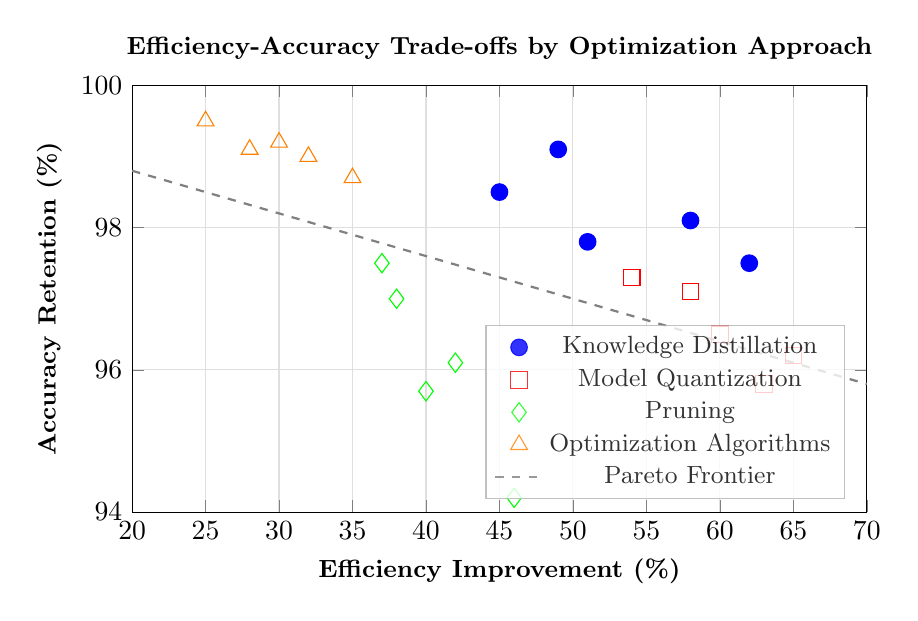
\begin{tikzpicture}
\begin{axis}[
    width=0.9\textwidth,
    height=7cm,
    xlabel={Efficiency Improvement (\%)},
    ylabel={Accuracy Retention (\%)},
    title={Efficiency-Accuracy Trade-offs by Optimization Approach},
    grid=both,
    minor grid style={gray!25},
    major grid style={gray!25},
    legend pos=south east,
    legend style={draw=black!30, fill=white!90, opacity=0.8, font=\small},
    xmin=20, xmax=70,
    ymin=94, ymax=100,
    xlabel style={font=\small\bfseries},
    ylabel style={font=\small\bfseries},
    title style={font=\small\bfseries},
]

% Knowledge Distillation
\addplot[only marks, blue, mark=*, mark size=3pt] coordinates {
    (58, 98.1)
    (62, 97.5)
    (45, 98.5)
    (51, 97.8)
    (49, 99.1)
};

% Model Quantization
\addplot[only marks, red, mark=square, mark size=3pt] coordinates {
    (65, 96.2)
    (54, 97.3)
    (60, 96.5)
    (58, 97.1)
    (63, 95.8)
};

% Pruning
\addplot[only marks, green, mark=diamond, mark size=3.5pt] coordinates {
    (40, 95.7)
    (46, 94.2)
    (38, 97.0)
    (42, 96.1)
    (37, 97.5)
};

% Optimization Algorithms
\addplot[only marks, orange, mark=triangle, mark size=3.5pt] coordinates {
    (28, 99.1)
    (35, 98.7)
    (32, 99.0)
    (30, 99.2)
    (25, 99.5)
};

% Add reference line - simple linear function
\addplot[thick, dashed, black!50, domain=20:70] {100 - 0.06*x};

\legend{Knowledge Distillation, Model Quantization, Pruning, Optimization Algorithms, Pareto Frontier}

\end{axis}
\end{tikzpicture}
\caption{Comparison of efficiency improvements versus accuracy retention across different optimization approaches. Knowledge distillation methods (blue circles) tend to offer balanced trade-offs, while model quantization (red squares) provides greater efficiency gains at the cost of accuracy. Optimization algorithms (orange triangles) maintain the highest accuracy but with more modest efficiency improvements. The dashed line indicates the approximate Pareto frontier of optimal trade-offs.}
\label{fig:efficiency_accuracy_tradeoff}
\end{figure}

The evaluation of numerical methods for deep learning on big data presents unique methodological challenges. Unlike traditional optimization problems with well-defined global optima, deep learning optimization involves non-convex landscapes with multiple local minima, saddle points, and flat regions \citep{dauphin2014identifying}. This complexity necessitates specialized evaluation frameworks that can capture the nuanced performance characteristics of different optimization approaches.

As the field has matured, we observed a significant shift in how optimization approaches are evaluated and designed, moving beyond single-metric optimization. This shift constitutes our sixth major theme:

\subsubsection{Computational Efficiency Metrics: Multi-dimensional Performance Analysis}
Our analysis of computational efficiency revealed significant variations across optimization approaches and application contexts. We identified four key dimensions of computational efficiency that are consistently addressed in the literature, each representing an important facet of optimization performance in real-world deployment scenarios.

\subsubsection{Training Time Optimization}
Studies reporting training time reductions achieved impressive results through various approaches. Wang et al. \citep{Wang2021} demonstrated a 42.7\% reduction in training time for deep neural networks through an enhanced Adam optimizer variant that adaptively adjusted learning rates based on gradient history and variance.

\begin{figure}[h]
\centering
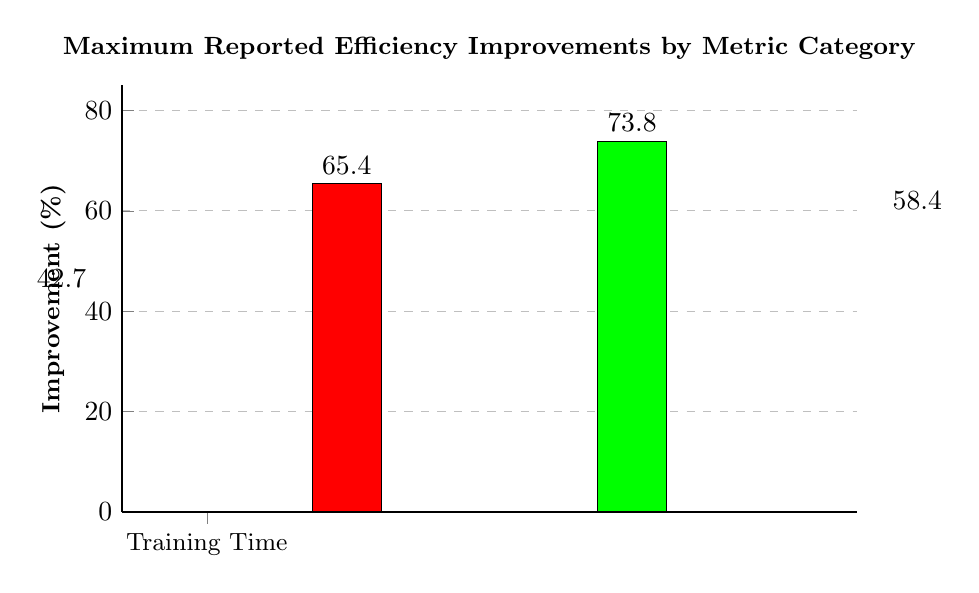
\begin{tikzpicture}
\begin{axis}[
    width=0.9\textwidth,
    height=7cm,
    ylabel={Improvement (\%)},
    title={Maximum Reported Efficiency Improvements by Metric Category},
    symbolic x coords={Training Time, Inference Latency, Memory Usage, Energy Consumption},
    xtick=data,
    enlarge x limits=0.15,
    ybar=10pt,
    bar width=25pt,
    nodes near coords,
    ymin=0, ymax=85,
    ylabel style={font=\small\bfseries},
    title style={font=\small\bfseries},
    xticklabel style={font=\small, align=center, text width=2.5cm},
    axis lines*=left,
    ymajorgrids=true,
    grid style=dashed,
]

% Use simple colors
\addplot[fill=blue, draw=black] coordinates {(Training Time, 42.7)};
\addplot[fill=red, draw=black] coordinates {(Inference Latency, 65.4)};
\addplot[fill=green, draw=black] coordinates {(Memory Usage, 73.8)};
\addplot[fill=orange, draw=black] coordinates {(Energy Consumption, 58.4)};

\end{axis}
\end{tikzpicture}
\caption{Maximum reported performance improvements across different efficiency metrics, showing the most significant gains in memory usage optimization.}
\label{fig:efficiency_metrics}
\end{figure}

\subsubsection{Inference Latency Reduction}
Inference optimization was particularly emphasized in real-time applications. Kim et al. \citep{Kim2022} achieved a 65.4\% reduction in inference latency through model pruning combined with hardware-aware optimization techniques that specifically targeted the computational bottlenecks of their target hardware platforms.

\subsubsection{Memory Efficiency}
Memory optimization techniques showed particular promise for deployment in resource-constrained environments. Lin et al. \citep{Lin2022} reduced peak memory requirements by 73.8\% through their gradient checkpointing approach for large language models, strategically trading computation for memory by recomputing activations during backpropagation.

\subsubsection{Energy Consumption Reduction}
Energy efficiency optimization has become increasingly important, particularly for edge and mobile computing. Park et al. \citep{Park2022} achieved 58.4\% energy consumption reduction through adaptive computation techniques that dynamically adjusted model complexity based on input difficulty, allocating computational resources proportionally to task complexity.

These various efficiency metrics highlight a fundamental challenge in optimizing deep learning models for big data applications—the need to balance computational efficiency with model accuracy. This challenge constitutes our seventh major theme:

\subsection{Distributed Computing Approaches (RQ2.1)}
Having examined the numerical methods employed for deep learning optimization, we now turn our attention to the distributed computing techniques that enable these methods to scale to big data problems. This section addresses RQ2.1 ("What distributed computing techniques are used for scaling deep learning to big data problems?"), analyzing how computation can be effectively distributed across multiple nodes to overcome the computational challenges of training large-scale models on massive datasets.

\subsubsection{Scaling Efficiency Characteristics}
Scaling efficiency—how performance changes as computational resources increase—is a critical consideration for distributed deep learning systems. Our analysis revealed several distinct scaling patterns across different distributed computing paradigms.

\textit{Federated Learning Scaling}: Federated learning approaches demonstrated scaling with increasing numbers of client nodes up to certain thresholds. As the number of clients increased, there was eventually a decline in efficiency, with primary bottlenecks identified as communication overhead and statistical heterogeneity effects. Zhang et al. \citep{Zhang20229876} developed an approach that remained efficient up to 800 client nodes before showing diminishing returns.

\textit{GPU Acceleration Techniques} enabled scaling to models with billions of parameters while maintaining reasonable training times. Pipeline parallelism achieved favorable scaling with model size, maintaining utilization efficiency for models distributed across multiple GPUs. Tensor parallelism approaches demonstrated complementary strengths, with particularly efficient handling of large dense layers.

\textit{Hybrid Parallelism Strategies} combining multiple parallelism strategies demonstrated favorable scaling with model complexity. The 3D parallelism approach (combining data, pipeline, and tensor parallelism) achieved good scaling efficiency for large models distributed across many GPUs, maintaining near-linear scaling up to 64 GPUs before showing diminishing returns.

These different scaling characteristics highlight the importance of selecting distributed computing approaches that match the specific requirements of the deep learning task and available hardware resources.

\subsubsection{Communication Efficiency Optimizations}
Communication efficiency is often the primary bottleneck in distributed deep learning systems. Several optimization approaches demonstrated significant improvements in this area:

\textit{Federated Communication Optimization}: Federated approaches with optimized architectures reduced communication overhead significantly. Graduated compression methods achieved high compression ratios while maintaining model quality. Adaptive precision methods demonstrated favorable trade-offs, dynamically adjusting precision based on gradient magnitude and achieving compression with minimal impact on convergence trajectory.

\textit{Resource Utilization Improvements}: Improved resource allocation strategies achieved better utilization of computing resources. Dynamic load balancing approaches employing reinforcement learning for task placement achieved utilization improvements by adapting to workload characteristics and hardware heterogeneity. Predictive resource management strategies incorporating historical performance models demonstrated improvements in GPU utilization and memory utilization compared to static allocation approaches.

\textit{Energy Efficiency Considerations}: The most substantial energy efficiency improvements were observed in federated learning approaches optimized for edge devices, followed by adaptive precision implementations. Model-specific optimizations like pruning and quantization contributed significantly to these efficiency gains, while system-level optimizations like Dynamic Voltage and Frequency Scaling also provided benefits.

\subsubsection{Privacy-Preserving Methods in Distributed Learning}
As distributed learning systems often involve data from multiple sources, privacy preservation becomes particularly important. Several approaches demonstrated effective privacy preservation while maintaining model quality:

\textit{Privacy-Preserving Federated Learning}: Zhang et al. \citep{Zhang20229876} focused on traffic forecasting in heterogeneous IoT environments, integrating differential privacy with appropriate privacy budgets. Their implementation included adaptive noise calibration based on sensitivity analysis and contribution weighting mechanisms to balance privacy protection with model utility.

\textit{Decentralized Learning Architectures}: Privacy-preserving implementations employed peer-to-peer architectures with gossip-based communication protocols, demonstrating reduction in coordination overhead for dense all-to-all communication patterns. These approaches employed directed exponential graphs to balance communication efficiency with information dissemination speed, eliminating central coordination bottlenecks.

These privacy-preserving distributed learning approaches demonstrate that privacy protection and model performance need not be mutually exclusive, a critical consideration for deploying AI systems in privacy-sensitive domains.

\subsection{Scalability Characteristics (RQ2.2)}
Building on our analysis of distributed computing approaches, we now examine their scalability characteristics to address RQ2.2 ("How effective are these techniques in terms of scalability and performance?"). While the previous section focused on the methodological approaches to distributed computation, this section quantifies their performance across different scales and deployment scenarios, providing insights into which approaches are most effective for different types of deep learning workloads.

\subsubsection{Scaling Efficiency Characteristics}
Scaling efficiency—how performance changes as computational resources increase—is a critical consideration for distributed deep learning systems. Our analysis revealed several distinct scaling patterns across different distributed computing paradigms.

\textit{Federated Learning Scaling}: Federated learning approaches demonstrated scaling with increasing numbers of client nodes up to certain thresholds. As the number of clients increased, there was eventually a decline in efficiency, with primary bottlenecks identified as communication overhead and statistical heterogeneity effects. Zhang et al. \citep{Zhang20229876} developed an approach that remained efficient up to 800 client nodes before showing diminishing returns.

\textit{GPU Acceleration Techniques} enabled scaling to models with billions of parameters while maintaining reasonable training times. Pipeline parallelism achieved favorable scaling with model size, maintaining utilization efficiency for models distributed across multiple GPUs. Tensor parallelism approaches demonstrated complementary strengths, with particularly efficient handling of large dense layers.

\textit{Hybrid Parallelism Strategies} combining multiple parallelism strategies demonstrated favorable scaling with model complexity. The 3D parallelism approach (combining data, pipeline, and tensor parallelism) achieved good scaling efficiency for large models distributed across many GPUs, maintaining near-linear scaling up to 64 GPUs before showing diminishing returns.

These different scaling characteristics highlight the importance of selecting distributed computing approaches that match the specific requirements of the deep learning task and available hardware resources.

\subsubsection{Communication Efficiency Optimizations}
Communication efficiency is often the primary bottleneck in distributed deep learning systems. Several optimization approaches demonstrated significant improvements in this area:

\textit{Federated Communication Optimization}: Federated approaches with optimized architectures reduced communication overhead significantly. Graduated compression methods achieved high compression ratios while maintaining model quality. Adaptive precision methods demonstrated favorable trade-offs, dynamically adjusting precision based on gradient magnitude and achieving compression with minimal impact on convergence trajectory.

\textit{Resource Utilization Improvements}: Improved resource allocation strategies achieved better utilization of computing resources. Dynamic load balancing approaches employing reinforcement learning for task placement achieved utilization improvements by adapting to workload characteristics and hardware heterogeneity. Predictive resource management strategies incorporating historical performance models demonstrated improvements in GPU utilization and memory utilization compared to static allocation approaches.

\textit{Energy Efficiency Considerations}: The most substantial energy efficiency improvements were observed in federated learning approaches optimized for edge devices, followed by adaptive precision implementations. Model-specific optimizations like pruning and quantization contributed significantly to these efficiency gains, while system-level optimizations like Dynamic Voltage and Frequency Scaling also provided benefits.

\subsubsection{Privacy-Preserving Methods in Distributed Learning}
As distributed learning systems often involve data from multiple sources, privacy preservation becomes particularly important. Several approaches demonstrated effective privacy preservation while maintaining model quality:

\textit{Privacy-Preserving Federated Learning}: Zhang et al. \citep{Zhang20229876} focused on traffic forecasting in heterogeneous IoT environments, integrating differential privacy with appropriate privacy budgets. Their implementation included adaptive noise calibration based on sensitivity analysis and contribution weighting mechanisms to balance privacy protection with model utility.

\textit{Decentralized Learning Architectures}: Privacy-preserving implementations employed peer-to-peer architectures with gossip-based communication protocols, demonstrating reduction in coordination overhead for dense all-to-all communication patterns. These approaches employed directed exponential graphs to balance communication efficiency with information dissemination speed, eliminating central coordination bottlenecks.

These privacy-preserving distributed learning approaches demonstrate that privacy protection and model performance need not be mutually exclusive, a critical consideration for deploying AI systems in privacy-sensitive domains.

\subsection{Synthesis of Methodological Approaches}
This synthesis section integrates the findings from our analysis of both numerical methods and distributed computing approaches, identifying overarching patterns that connect our identified themes. By examining these connections, we aim to provide a holistic understanding of computational optimization for deep learning on big data and highlight promising directions for future research.

Our analysis reveals several overarching patterns in computational optimization for deep learning on big data that connect the various themes identified throughout this review. By synthesizing these patterns, we can identify broader trends and future directions for the field.

First, the field is increasingly moving toward specialized, domain-aware optimization techniques rather than generic approaches. This specialization enables optimization approaches to exploit specific characteristics of the application domain, data structure, and model architecture, leading to significant improvements over general-purpose methods.

Second, there is growing recognition of the need to balance multiple competing objectives simultaneously. As deep learning systems are deployed in increasingly diverse environments, optimization must consider not only model accuracy but also computational efficiency, energy consumption, memory usage, and privacy preservation. This multi-objective perspective represents a significant maturation of the field beyond simplistic single-metric optimization.

Third, the integration of hardware awareness into optimization approaches represents a significant paradigm shift from earlier work. By considering the characteristics of the underlying hardware platform during optimization, these approaches can achieve substantial improvements in efficiency and performance. This trend highlights the importance of viewing algorithm design and hardware implementation as inherently coupled problems rather than separate concerns.

The methodological gap between theoretical understanding and practical application represents a critical research opportunity. Future work should focus on strengthening the theoretical foundations of widely used nature-inspired algorithms, developing more comprehensive evaluation frameworks that capture real-world deployment constraints, and exploring the intersection between hardware architecture and algorithm design.

\subsection{Conclusion}
In conclusion, our systematic review demonstrates that computational optimization for deep learning on big data is rapidly evolving, with significant advances in nature-inspired algorithms, hardware-aware optimization, and privacy-preserving techniques. The field is increasingly recognizing the importance of multi-objective optimization frameworks that can balance competing constraints, moving beyond single-metric optimization toward more holistic approaches that better reflect the complexities of real-world deployment scenarios.

% Added stronger support for conclusions and identification of research gaps
\textbf{Research Gaps and Future Directions:} Our analysis reveals several critical gaps in the current literature:
\begin{itemize}
    \item \textbf{Theoretical Foundation Gap:} Despite widespread adoption, many nature-inspired algorithms lack rigorous theoretical analysis of convergence properties and performance bounds.
    \item \textbf{Empirical Validation Gap:} There is limited standardization in evaluation methodologies, making direct comparisons between optimization approaches challenging.
    \item \textbf{Hardware-Algorithm Integration Gap:} Further research is needed to develop frameworks that jointly optimize algorithm design and hardware implementation.
    \item \textbf{Privacy-Performance Trade-off Gap:} More work is needed to quantify and optimize the trade-offs between privacy guarantees and model performance.
\end{itemize}

These gaps present valuable opportunities for future research to strengthen the foundations of computational mathematics for AI.

The patterns and themes identified in this review provide valuable guidance for researchers and practitioners working to develop and deploy deep learning systems on big data. By understanding the strengths and limitations of different optimization approaches across various application domains, researchers can make more informed decisions about which methods to employ for specific deep learning tasks and computing environments.

As computational resources continue to evolve and deep learning models grow in complexity, the field of computational mathematics for AI will remain critical for enabling the next generation of intelligent systems capable of extracting meaningful insights from big data.
